% ********** Chapter 5 **********
\chapter{Connection Specification}
\label{chapter5}

This chapter aim to give a complete description of the behaviour of this connection. Thus, a description of each part of this connection will be given and the interaction with the users will be explored. In order to better understand this connection, it will be decomposed into well defined logical components. Each component will have its own interfaces defined in order to understand how the communication between those components works. Together with the explanation, this connection will also be illustrated through figures of each component, with particular emphasis on the component describing the mapper between \vpp\ and \jml.

\section{Overview}

After completing the previous steps described in chapter \ref{chapter4}, one will have ASTs representing input files. In order to map specifications both from \vpp\ and \jml, a mapper should be defined. This mapper should be able to convert \vpp\ ASTs into \jml\ ASTs and vice-versa. In virtue of the ASTs store all the necessary information in order to convert to other ASTs representing the target language. However, such a conversion should respect the semantic rules defined in chapter \ref{chapter3}, in order to maintain the semantic value of the languages.

Such a mapper should allow one to move freely from \vpp\ to \jml\ and vice-versa. However, there will be a pre-processor responsible to check if it possible to preform the connection, based on the semantic rules of both languages.

The referred pre-processor is explained in detail in section \ref{chap5:preproc}. Furthermore, in section \ref{chap5:state} one can see the specification and corresponding explanation of the state information. Finally, in section \ref{chap5:mapper} one can see some of the key operations of the specification of the mapper both from \vpp\ to \jml\ and \jml\ to \vpp. Note that the pre-processor and the state information are only necessary when moving from \vpp\ to \jml, thus the explanations will be focused on this assumption.


\section{Pre-processor}
\label{chap5:preproc}

The pre-processor component of this specification if of great importance concerning the mapper from \vpp\ to \jml. As it can be seen from chapter \ref{chapter3}, there are three key situations where \vpp\ specifications should be pre-processed: 
\begin{itemize}
\item If there exists multiple inheritance, it should be resolved because \jml\ does not allow multiple inheritance;
\item If there is type information in the specification, which is not a composite type, it should be saved into an intermediate structure in order to consult the name of the type at the \jml\ side; and
\item Whenever a \vpp\ specification has composite type definitions, a new class should be created to each of those composite types.
\end{itemize}

Each of these three points will be explained in detail below. A number of operations from the \vpp\ specification of the pre-processor are shown to illustrate how these concepts are used in practice.

Starting with the multiple inheritance issue, it is necessary to resolve it when moving from \vpp\ to \jml. The adopted solution was explained in subsection \ref{chap2:sec:inh}, and it is illustrated in figure \ref{chap5:figure:pre}. In figure \ref{chap5:figure:pre}, the parsing component of \vpp\ is omitted. The ASTs will then be pre-processed by the pre-processor. That component will initially check if there is any multiple inheritance present. 

\begin{figure}[!htb]
\begin{center}
\resizebox{.99\textwidth}{!}{\includegraphics{chap5/preprocessor.ps}}
\end{center}
\caption{Illustration of the pre-processor over VDM++ specifications.}
\label{chap5:figure:pre}
\end{figure}

In case there are no multiple inheritance, the pre-processor will gather type and class information into a state component, which is explained in section \ref{chap5:state}, and it start the mapper component, explained in section \ref{chap5:mapper}. 

On the other hand, if there is multiple inheritance, the pre-processor will try so resolve it, \ie, it will try to eliminate the multiple inheritance applying the rules explained in section \ref{chap2:sec:inh}. If it is not possible to satisfy the referred rules, the pre-processor will finish its execution and the mapper will not run because it would generate erroneous classes, with multiple inheritance, which is not supported at the \jml\ side. 

However, if it is possible to eliminate the multiple inheritance, the pre-processor will eliminate it, gather type and class information and finally it will proceed to the mapping component. Note that the elimination of the multiple inheritance will consist in mapping one or more classes into interfaces. That information will also hold in the state information, as explained in section \ref{chap5:state}. That information will then be used by the mapper for further treatment.

The operations responsible for this are presented below. The operation \textit{init} is the responsible for activating the pre-processor in order to understand if there is any multiple inheritance.
\lstset{style=mystyle}
\bigskip
\begin{lstlisting}
public init :
  OmlSpecifications ==>
  JmlSpecifications
init(specs) ==
  if preprocess(specs) 
  then return eliminateMI(specs)
  else return build_jml(specs);
\end{lstlisting}
\bigskip
If the specifications have multiple inheritance, the pre-processor tries to eliminate it through the following operation:
\bigskip
\begin{lstlisting}
public eliminateMI : 
  OmlSpecifications ==>
  JmlSpecifications
eliminateMI(specs) == 
  if canProceed(specs)
  then (eliminate(specs);
        build_jml(specs))
  else return new JmlSpecifications([]);
\end{lstlisting}
\bigskip
This operation will call the operation \textit{canProceed} which will try to see if it is possible to eliminate the multiple inheritance. This is preformed by checking if at most one of the superclasses of the class in question is a class and if all the other superclasses can be transformed into interfaces.

Finally, if it is possible to eliminate the multiple inheritance, the \textit{eliminate} operation will update the state information in order to be used by the mapper. Below, one can see the mentioned operation:
\bigskip
\begin{lstlisting}
public eliminate :  
  OmlSpecifications ==>
  ()
eliminate(specs) == 
  (interfaces_list := updateInterfaceList(specs);
   classes_list := updateClassList(specs));
\end{lstlisting}
\bigskip

The operations that checks if a given class has multiple inheritance is the operation \textit{hasMI}, and its specification is presented below:
\bigskip
\begin{lstlisting}
public hasMI :
  OmlClass ==>
  bool
hasMI(c) == 
  let ic = c.getInheritanceClause()
  in if c.hasInheritanceClause()
     then let l = len ic.getIdentifierList()
	      in if l > 1 
			 then return true
     else return false
	 else return false;
\end{lstlisting}
\bigskip
It will check if a given class has more than one superclass, and it will return the verdict: \textit{true} if it has mutliple inheritance and \textit{false} if it has no multiple inheritance.

\section{State Information}
\label{chap5:state}

In order to be able to preform the mapping between the two specification languages in an efficient way, it is important to gather a number of relevant information before mapping the ASTs. Afterwards, the mapper will then access that state information in order to preform actions such as decide about inheritance and resolve type names.

The state information showed in figure \ref{chap5:figure:pre} is composed by the following elements:
\begin{itemize}
\item A set of strings, representing \vpp\ class names that will become classes in \jml ;
\item A set of strings, representing \vpp\ class names that will become interfaces in \jml ;
\item A mapping, where the domain elements is composed by class names and the range elements is composed again another map with information relative to type information;
\item Finally, another map where the domain is composed by class names and the range is composed by type information (complex \vpp\ types) that will be transformed into classes in \jml .
\end{itemize}
The components mentioned are instance variables that will hold a number of information that will be supplied to the mapper during the transformations. The \vpp\ types can be seen below.
\lstset{style=AST}
\bigskip
\begin{lstlisting}
types

public Information ::
  field_list : seq of JmlField
  invariant  : [JmlExpression];
public TypeInfo = map ClassId to JmlType;
public ClassId = seq of char;
\end{lstlisting}
\bigskip

With respect to the instance variables, the \vpp\ specification of then is showed below:

\bigskip
\begin{lstlisting}
instance variables

public to_class : map ClassId to Information;
public hold_type_info : map ClassId to TypeInfo;
public interfaces_list : set of ClassId;
public classes_list : set of ClassId;
\end{lstlisting}
\bigskip

The first two items, named \textit{interfaces\_list} and \textit{classes\_list}, represents sequences of class names that will become classes or interfaces in \jml. Those structures will hold the information gathered by the pre-processor about multiple inheritance. Thus, the pre-processor will first make sure if it is possible to solve the multiple inheritance, and afterwards, if it is possible, it will fill those sequences with the correct information promoting the necessary classes to interfaces and maintaining the others as classes. Whenever the mapper needs to update the information about inheritance of a given class, it will consult the two sets in order to adjust the information correctly. 

The operation responsible for updating this information is the operation \textit{eliminate} presented in section \ref{chap5:preproc}.

The third item showed above, named \textit{hold\_type\_info}, is a map from \vpp\ class names to type information. In \vpp\ the creation of simple types, which are types with an identifier and a type based on the pre-defined types in \vpp, is common. One example of those types can be found below:
\lstset{style=mystyle}
\bigskip
\begin{lstlisting}
types

public String = seq of char;
\end{lstlisting}
\bigskip
In this example, the type \textit{String} is created by means of a pre-defined type in \vpp which is a sequence of characters. Afterwards, if one uses the created type inside, for example, an operation like the following:
\bigskip
\begin{lstlisting}
operations

public concat : String * String ==> String
concat(s1,s2) == is not yet specified;
\end{lstlisting}
\bigskip
Then, the mapper needs to know what is the \vpp\ type behind the keyword \textit{String}, in order to make the transformations to a \jml\ type. To preform this, the pre-processor will gather this kind of information. Each class named will be mapped into another map, where the key values are type names (in this example, \textit{String}) and the range will be the corresponding \vpp\ type already transformed into a \jml\ type. In this case, because the \textit{seq of char} is equivalent to the \jml\ type \textit{JMLValueSequence}, the \jml\ type will be placed as the range of the \textit{String}. Thus, whenever the type name \textit{String} is used, the mapper will consult the mapping in order to obtain the type behind the keyword that identifies it.

Finally, with respect to the fourth instance variable named \textit{to\_class}, whenever a class has complex types, they should be mapped into \jml\ classes due to the fact they have fields and possible invariants. If there is a type with an invariant such as:
\lstset{style=AST}
\bigskip
\begin{lstlisting}
types

public PairOfNat ::
  fst : nat
  snd : nat
inv t == t.fst < t.snd;
\end{lstlisting}
\bigskip

Then, the final map will contain, for the class in question, the information regarding the type \textit{PairOfNat}, where the type name will be the domain and in the range there will be a list of fields and possibly an invariant. In this case, the list of fields will hold the information regarding the fields \textit{fst} and \textit{snd} and the type information associated, already converted to the correspondent \jml\ types. Besides that, because the type has an invariant associated, its expression will be transformed into an equivalent \jml\ expression representing the invariant, and that information will be saved together with the field list. Note that the operation returns always a \textit{true} value, because it is being used inside a sequence comprehension, which requires the operation to return.
\lstset{style=mystyle}
\lstset{language=VDM++}
\bigskip
\begin{lstlisting}
public buildClassEntry :
  OmlClass ==>
  bool
buildClassEntry(c) ==
  let cn = c.getIdentifier(),
      bl = c.getClassBody(),
      ts = buildTypeInfo(bl),
      cl = toClassInformation(bl)
  in (
        hold_type_info := hold_type_info ++ { cn |-> ts };
        to_class := to_class ++ cl;
        return true;
     );
\end{lstlisting}
\bigskip

After the pre-processor gathers all the relevant information, the mapper is ready to convert the two specifications languages. Afterwards, if there are type information that should be mapped into classes, it should be performed by a post-processor over the type information gathered in the instance variable \textit{to\_class}.

\section{Mapper}
\label{chap5:mapper}

After performing the actions described in sections \ref{chap5:preproc} and \ref{chap5:state}, the mapper is ready to be used. The goal of this mapper is to convert ASTs from \jml\ to \vpp\ and vice-versa. As it was said above, the pre-processor will only be needed when moving from \vpp\ to \jml. Besides this, the two mappers are very similar, and their goal is to map a number of constructs using the abstract syntax defined in \vdm, as it can be seen from appendix \ref{appendix:jmlast}. A number of relevant operations that perform such transformations is presented in the subsections below. Figure \ref{chap5:figure:map} illustrates the mapper functionality, and as it can be seen, it suggests a link comming from the pre-processor figure \ref{chap5:figure:pre}.

\begin{figure}[!htb]
\begin{center}
\resizebox{.99\textwidth}{!}{\includegraphics{chap5/mapper.ps}}
\end{center}
\caption{Illustration of the mapper functionality.}
\label{chap5:figure:map}
\end{figure}

\subsection{Mapper from \vpp\ to \jml}
\label{chap5:secmap:subvppjml}

The main operation of this mapper, called \textit{build\_jml}, is the responsible for mapping each class present in the AST into \jml\ classes.

\bigskip
\begin{lstlisting}
public build_jml : 
  OmlSpecifications ==> 
  JmlSpecifications
build_jml(specs) == 
  let classes = specs.getClassList(),
      jml_classes = convertVdm2JmlClasses(classes)
  in return new JmlSpecifications(jml_classes);
\end{lstlisting}
\bigskip
As it can be seen, the operations transforms each class into a \jml\ class. The operation responsible for mapping a \vpp\ class into a \jml\ class is the following:
\bigskip
\begin{lstlisting}
 public convertVdm2JmlClass : 
  OmlClass ==> 
  JmlWrappedJmlClass
convertVdm2JmlClass(c) == 
  let id   = c.getIdentifier(),
	  inh  = c.getInheritanceClause(),
      body = c.getClassBody(),
      jmlclass = build_class(id, inh, body),
      jmlimp = getJmlImports(),
      javaimp = getJavaImports()
  in return new JmlWrappedJmlClass([],[],javaimp,jmlimp,jmlclass);
\end{lstlisting}
\bigskip
The subsequent operations are similar, and the goal is to map construct by construct, respecting the rules already defined and the limitations encountered. From those operations, there is a number of them responsible for the main blocks present in a \vpp\ specification.

The values block inside a \vpp\ specification is mapped into a similar values block in \jml, which represents static variables inside the code. Thus, each value in a \vpp\ specification is mapped into a static variable in \jml\ by means of the operation \textit{buildJmlValue}, presented below:

\bigskip
\begin{lstlisting}
public buildJmlValue : 
  OmlValueDefinition ==> 
  JmlValueDefinition
buildJmlValue(val) == 
  let access = val.getAccess(),
      shape = val.getShape(),
      newAccess = buildJmlAccess(access),
      newShape = buildJmlShape(shape)
  in return new JmlValueDefinition(newAccess,true,true,newShape);
\end{lstlisting}
\bigskip

Furthermore, each instance variable in a \vpp\ class is mapped into a \jml\ variable by means of the following operation:
\bigskip
\begin{lstlisting}
public buildVariables : 
  OmlInstanceVariable ==> 
  JmlVariable
buildVariables(var) == 
  let access = var.getAccess(),
      scope = access.getScope(),
      assign = var.getAssignmentDefinition(),
      newScope = new JmlScope(scope.getValue()),
      newAccess = new JmlAccessDefinition(newScope),
      stat = access.getStaticAccess(),
      tp = convertType(assign.getType()),
      id = assign.getIdentifier(),              
      expr = convertExpression(assign.getExpression())
  in return new JmlVariable(newAccess, true, stat, 
                            false, tp, id, expr);
\end{lstlisting}
\bigskip
This operation will gather all the information necessary to convert a \vpp\ instance variable into a \jml\ variable. Moreover, each operation in \vpp\ is mapped into a \jml\ operation using one of three operations, because it is possible to have three kinds of operations in \vpp : implicit, explicit and extended explicit. As an example, the operation that converts an explicit \vpp\ operation into a \jml\ operation is showed below:

\bigskip
\begin{lstlisting}
public buildExplicitJmlOperation : 
  JmlAccessDefinition * 
  bool *
  OmlExplicitOperation ==>
  JmlOperationDefinition
buildExplicitJmlOperation(access,statickey,shape) == 
  let id = shape.getIdentifier(),
      tp = shape.getType(),
      type_rng = getRngType(tp),
      params = shape.getParameterList(),
      trailer = buildOperationTrailer(shape.getTrailer(),access),
      paramsList = buildOperationParameters(params,tp)
  in return new JmlOperationDefinition(trailer,access,true,
     statickey,false,type_rng,id,paramsList,nil);
\end{lstlisting}
\bigskip
Besides the operation, all its trailers, \ie, pre-, post-conditions, error and external clauses are also mapped by means of the operation \textit{buildOperationTrailer}, provided in appendix \ref{appendix2}. 

With respect to types, they are mapped using operations such as the following one, that converts a \vpp\ product type into a \jml\ tuple type, created to hold this kind of information.

\bigskip
\begin{lstlisting}
public convertProductType :
  OmlProductType ==>
  JmlTupleType
convertProductType(t) ==
  let tp = buildSeqTypes(t),
      sq = [ convertType(tp(i)) | i in set inds tp ]
  in return new JmlTupleType(sq);
\end{lstlisting}
\bigskip
Any other \vpp\ block used in a \vpp\ class will be ignored, and thus it will not be mapped.

Although the following conversions are not between blocks, they are essential to the entire mapping. This conversions are between expressions and literals. Expressions are present in every sentence of a language, and they are connected by means of operations such the following, that converts a \jml\ \textit{let} expression into a definition block in \jml :

\bigskip
\begin{lstlisting}
public convertLetExpression :
  OmlLetExpression ==>
  JmlBlockExpression
convertLetExpression(e) ==
  let bind = e.getDefinitionList(),
      newbind = buildJmlShapes(bind),
      expr = e.getExpression(),
      res = convertExpression(expr)
  in return new JmlBlockExpression(newbind,res);
\end{lstlisting}
\bigskip

There are a number of similar operations responsible for converting a number of \vpp\ expressions into \jml\ expressions, which are listed and explained in appendix \ref{appendix2}.

Finally, literals allow one use elements of a give type. One example of an operation is as follows:
\bigskip
\begin{lstlisting}
public convertBooleanLiteral :
  OmlBooleanLiteral ==>
  JmlBooleanLiteral
convertBooleanLiteral(n) ==
  let val = n.getVal()
  in return new JmlBooleanLiteral(val);
\end{lstlisting}
\bigskip

The complete specification and description is presented in appendix \ref{appendix2}. The limitations that this mapper imposes were defined in chapter \ref{chapter3}. After performing the pre-processing stage and after running the mapper over \vpp\ ASTs, it is possible to have \jml\ ASTs ready to be pretty-printed into concrete classes. Examples of this mapper and the pre-processor can be found in chapter \ref{chapter6}. Two case studies were used in order to test the functionalities explained along this chapter.

\subsection{Mapper from \jml\ to \vpp}

This mapper from \jml\ to \vpp\ is similar to the one mentioned in subsection \ref{chap5:secmap:subvppjml}, with respect to the mapping of the ASTs. Concerning the pre-processing part, it is not required here because there are no limitations excepting the usage of constructs that are not being considered by this connection.

Thus, the main operation of this mapper is the operation \textit{build\_vdm}, presented below.

\lstset{style=mystyle}
\bigskip
\begin{lstlisting}
public build_vdm : 
  JmlSpecifications ==>
  OmlSpecifications
build_vdm(specs) ==
  let classes = specs.getClassList(),
      vdmclasses = convertJmlClasses(classes)
  in return new OmlSpecifications(vdmclasses);
\end{lstlisting}
\bigskip

This operation will transform each \jml\ specification received as input into a correspondent specification in \vpp. Each specification has a class list, and the operation that transforms each \jml\ class into a \vpp\ class is the following:

\lstset{style=mystyle}
\bigskip
\begin{lstlisting}
public convertJmlClass :
  JmlWrappedJmlClass ==>
  OmlClass
convertJmlClass(c) ==
  let cl = c.getClassVal(),
      id = cl.getIdentifier(),
      ic = cl.getInheritanceClause(),
      ii = cl.getInterfaceInheritance(),
      ih = getInheritanceClauses(ic,ii),
      bd = cl.getClassBody(),
      body = convertClassBody(bd)
  in return new OmlClass(id,[],ih,body,false);
\end{lstlisting}
\bigskip

Further on, it is necessary to transform each \jml\ block into a \vpp\ block (e.g., operations block). Below, a number of operations responsible for the transformation of each considered block is presented and explained.

Starting with the operation named \textit{convertInstanceVariables}, it converts \jml\ instance variables into \vpp\ instance variables. The other operations in use are listed and explained in appendix \ref{appendix2}.

\bigskip
\begin{lstlisting}
public convertInstanceVariables :
  JmlInstanceVariableDefinitions ==>
  OmlInstanceVariableDefinitions
convertInstanceVariables(s) == 
  let jml_vars = s.getJmlVariables(),
      java_vars = s.getJavaVariables(),
	  vdm_1 = convertVariables(jml_vars),
	  vdm_2 = convertVariables(java_vars),
	  res = vdm_1 ^ vdm_2
  in return new OmlInstanceVariableDefinitions(res);
\end{lstlisting}
\bigskip

Furthermore, the operation \textit{convertValueDefinitions} converts \jml\ values into \vpp\ values. The specification of the referred operation is as follows:

\bigskip
\begin{lstlisting}
public convertValueDefinitions :
  JmlValueDefinitions ==>
  OmlValueDefinitions
convertValueDefinitions(s) == 
  let l = s.getValueList(),
      q = convertValues(l)
  in return new OmlValueDefinitions(q);
\end{lstlisting}
\bigskip

The invariant definition present in \jml\ are mapped into \vpp\ invariants applied to instance variables, \ie, they are written as instance variables invariants within the instance variables block. The operation responsible for such transformation is shown below.

\bigskip
\begin{lstlisting}
public convertInvariantDefinitions :
  JmlInvariantDefinitions ==>
  OmlInstanceVariableDefinitions
convertInvariantDefinitions(s) == 
  let l = s.getInvariantList(),
      q = convertInvariants(l)
  in return new OmlInstanceVariableDefinitions(q);
\end{lstlisting}
\bigskip

With respect to operations, \jml\ operations are converted into \vpp\ implicit operations for two reasons:
\begin{itemize}
\item This connection does not connect methods implementations, thus there is no need to have explicit operations;
\item If a \jml\ operation has an assignable clause, which is equivalent to the \vpp\ external clause, it can only be mapped if the \vpp\ operation is implicit, because explicit operations does not allow the usage of such clause.
\end{itemize}
Thus, the operation responsible for converting a \jml\ operation into a \vpp\ implicit operation is the operation called \textit{convertOperation}.

\bigskip
\begin{lstlisting}
public convertOperation :
  JmlOperationDefinition ==>
  IOmlOperationDefinition
convertOperation(op) ==
  let access = op.getAccess(),
      stat = op.getStatickeyword(),
      newaccess = buildAccessDefinition(access,stat),
      id = op.getIdentifier(),
      t = op.getReturningType(),
      p = op.getParameterList(),
      tp = buildOperationType(t,p,id),
      params = buildParametersList(p),
      trl = op.getTrailer(),
      trailer = buildOperationTrailers(trl),
      shape = new OmlImplicitOperation(id,params,tp,trailer)
  in return new OmlOperationDefinition(newaccess,shape);
\end{lstlisting}
\bigskip

There are no other blocks being considered in this mapping from \jml\ to \vpp. However, it is still necessary to map types, expressions and literals. 

Starting with types, each \jml\ type that has a correspondence at the \vpp\ level is being mapped by means of operations such as the following operation, which converts a \jml\ map type to a \vpp\ map type.

\bigskip
\begin{lstlisting}
public convertMapType :
  JmlMapValueToValueType ==>
  OmlGeneralMapType
convertMapType(m) ==
  let domtp = m.getDomType(),
      rngtp = m.getRngType(),
	  tpd = convertType(domtp),
	  tpr = convertType(rngtp)
  in return new OmlGeneralMapType(tpd,tpr);
\end{lstlisting}
\bigskip

The other operations responsible for the conversion of the rest of the types are present in appendix \ref{appendix2}.

With respect to expressions, an example of converting a \jml\ expression into a \vpp\ expression can be found below.

\bigskip
\begin{lstlisting}
public convertBinaryExpression :
  JmlBinaryExpression ==>
  OmlBinaryExpression
convertBinaryExpression(e) ==
  let lhs = e.getLhsExpression(),
	  op  = e.getOperator(),
	  rhs = e.getRhsExpression(),
	  nlhs = convertExpression(lhs),
	  nop = convertBinaryOperator(op),
	  nrhs = convertExpression(rhs)
  in return new OmlBinaryExpression(nlhs,nop,nrhs);
\end{lstlisting}
\bigskip

The operation above converts a \jml\ binary expression into a \vpp\ binary expression, by means of other operations presented in appendix \ref{appendix2}.

Finally, the operation \textit{convertLiteral} is responsible to infer the input type in order to  assign the correspondent operation that will convert the literal expression.

\bigskip
\begin{lstlisting}
public convertLiteral :
  IJmlLiteral ==>
  IOmlLiteral
convertLiteral(lit) == 
  cases true:
    (isofclass(JmlNumericalLiteral,lit))
	  -> return convertNumericalLiteral(lit),
    (isofclass(JmlFloatLiteral,lit))
	  -> return convertFloatLiteral(lit),
    (isofclass(JmlEnumLiteral,lit))
	  -> return convertEnumLiteral(lit),
    (isofclass(JmlBooleanLiteral,lit))
	  -> return convertBooleanLiteral(lit),
    (isofclass(JmlCharacterLiteral,lit))
	  -> return convertCharacterLiteral(lit),
    (isofclass(JmlStringLiteral,lit))
	  -> return convertStringLiteral(lit),
	(isofclass(JmlNullLiteral,lit))
	  -> return new OmlNilLiteral(),
	others
	  -> return new OmlNilLiteral()
  end;
\end{lstlisting}
\bigskip


From this chapter, it was possible to see the procedures of the defined maped, and a number of operations responsible for converting between the two specification languages in question. More information about the specification in \vpp\ of this mapper can be found in appendix \ref{appendix2}.

% ********** End of chapter **********
